\clearpage

\begin{tcolorbox}	
\begin{tabular}{p{2.75cm} p{0.2cm} p{10.5cm}} 	
\textbf{Student Name}  &:& Tiago Esteves\\
\textbf{Starting Date} &:& October 03, 2017\\
\textbf{Goal}          &:& Implement the dimensioning of optical networks in the translucent transport mode.
\end{tabular}
\end{tcolorbox}

\section{Objective and methodology for the dissertation}

\subsection{Objective}
The objective of this dissertation is to develop ILP and Heuristic models for networks with translucent transport mode and finally integral in net2plan.
To achieve this goal, the following steps must be:
\begin{itemize}
  \item Develop ILP models for opaque, transparent and translucent networks using 1 + 1 protection.
  \item Obtain a solution for network through heuristic algorithms.
  \item Compare and validate the results obtained through the heuristics with the results based on ILP.
\end{itemize}

\subsection{Methodology}
The methodology used in this dissertation is to define two networks (a reference network and another realistic network) and then apply the ILPs to the reference network and to the realistic network.
Subsequently we will develop heuristics that will be generated in Net2Plan and validated based on the comparison with the results obtained from the ILPs.
In addition to being used two networks will also be applied two possible scenarios being one of them with little traffic and the other with much traffic.

This procedure will be done as follows:
\begin{enumerate}
  \item Opaque with 1+1 Protection
  \item Transparent with 1+1 Protection
  \item Translucent with 1+1 Protection
\end{enumerate}

\section{Physical Network Topology}

\subsection{Reference Network}
As we can see in the figure, our reference network consists of 6 nodes and 8 Bidirectional links.
The average length of the links was chosen so that the following calculations are more simplistic.

\begin{figure}[h!]
\centering
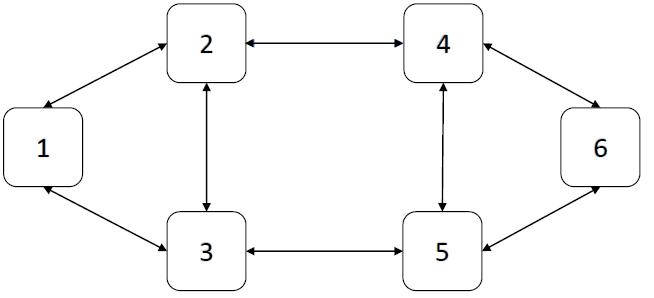
\includegraphics[width=\textwidth]{RedeTeste}
\caption{Physical Topology of the Reference Network.}
\end{figure}

\vspace{10pt}

The following table shows the values of the variables associated with this network.
\begin{table}[h!]
\vspace{10pt}
\centering
\begin{tabular}{|| c | c | c||}
 \hline
 Constant & Description & Value \\
 \hline\hline
 N & Number of Nodes & 6 \\
 L & Number of Bidirectional Links & 8 \\
 <$\delta$> & Node out-degree & 2,667 \\
 <len> & Mean Link Length (km) & 500 \\
 <h> & Mean Number of Hops,for Working Paths & 1,533 \\
 <h'> & Mean Number of Hops,for Backup Paths & 2,467 \\
 \hline
\end{tabular}
\caption{Table of reference network values}
\label{table:1}
\end{table}
\vspace{10pt}

As we can see from table \ref{table:1}, to do all the calculations necessary for this project, let us know the value of the traffic used. This value is defined depending on the scenario used, as we can see:
\begin{itemize}
  \item Shortly Traffic: \textbf{0.5 TBits/s}
  \item Very Traffic: \textbf{5 TBits/s}
\end{itemize}
\vspace{10pt}

\subsection{Realistic Network}
The real network chosen for this work is the EON (European Optical Network).
The way the nodes are arranged geographically can be seen from the following figure.
\vspace{100pt}

\begin{figure}[h!]
\centering
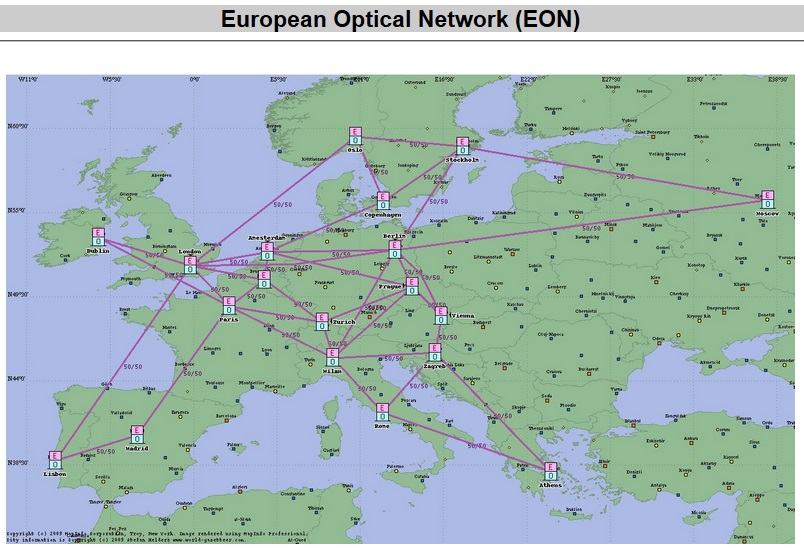
\includegraphics[width=\textwidth]{EON_Rede_Realista}
\caption{Physical Topology of the Realistic Network.}
\end{figure}

The table \ref{table:2} shows the values of the variables associated with this network.
\begin{table}[h!]
\centering
\begin{tabular}{|| c | c | c||}
 \hline
 Constant & Description & Value \\
 \hline\hline
 N & Number of Nodes & 19 \\
 L & Number of Bidirectional Links & 37 \\
 <$\delta$> & Node out-degree & 3,89 \\
 <len> & Mean Link Length (km) & 753,76 \\
 <h> & Mean Number of Hops,for Working Paths & 2,3 \\
 <h'> & Mean Number of Hops,for Backup Paths & 3,2 \\
 \hline
\end{tabular}
\caption{Table of realistic network values}
\label{table:2}
\end{table}
\vspace{10pt}

Again, to make all the necessary calculations, only the value of the traffic used is missing. This value is set depending on the scenario used, as we can see:

\begin{itemize}
  \item Shortly Traffic: \textbf{2 TBits/s}
  \item Very Traffic: \textbf{20 TBits/s}
\end{itemize}
\vspace{10pt}

\section{Dimensioning using ILP models}

\subsection{Opaque with 1+1 Protection}
The objective function of following ILP is a minimization of the sum of two variables: total number of flows crossing link (i; j) for all demand pairs (o; d) and total number of optical channels in each link (i; j).
\begin{figure}[h!]
  \centering
  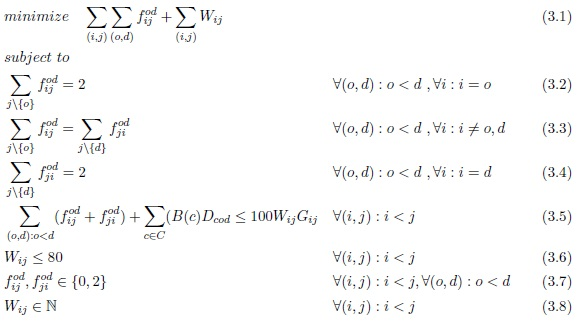
\includegraphics[scale=1]{ILP_Opaque}
\end{figure}

The objective function, to be minimized, is the expression(3.1). The flow conservation constraints are (3.2), (3.3) and (3.4). First constraint ensures that, for all demand pairs (o,d), it routes two flows of traffic for all bidirectional links (i,j) when "j" is not equal to the origin of the demand. Equation (3.4) is based on the same idea of (3.1), however applied in reverse direction. Assuming bidirectional traffic, so the number of flows in both directions of the link is the same (3.3). The inequality (3.5) is considered grooming constraint, so it means the total client traffic flows can not be greater than the capacity of optical channels on all links. Another important constraint (3.6) is the capacity of the optical channels which must be less or equal to 100 Gb/s or 80 ODU0. The number of flows per demand can be zero if there are no traffic demands or two if considering working and protection traffic (3.7). The last constraint is just needed to ensure the number optical of channels is a positive integer values greater than zero.

\subsection{Transparent with 1+1 Protection}

The optimization model suggested for transparent transport mode with dedicated path protection intends to minimize the total number of flows crossing link (i; j) for all demand pairs (o; d). The mathematical model described below also minimizes the total number of optical channels between each demand end nodes Wod, instead of minimizing the number of optical link-by-link channels as in the previous model.

\begin{figure}[h!]
  \centering
  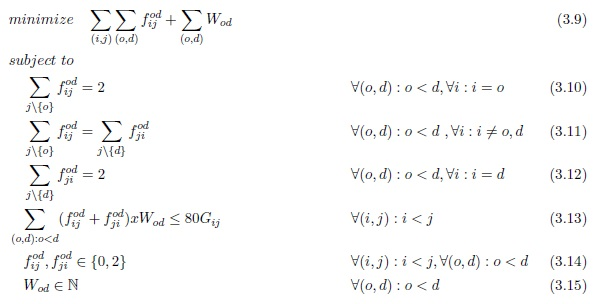
\includegraphics[scale=1]{ILP_Transp}
\end{figure}

The objective function, to be minimized, is the expression(3.9). The flow conservation is performed by equations (3.10), (3.11) and (3.12) and share the same mathematical description of opaque model. The inequality (3.13) answers capacity constraint problem. Then, total flows times the traffic of the demands must be less or equal to the capacity of network links. The grooming of this model can be done before routing since the traffic is aggregated just for demands between the same nodes, thus not depending on the routes. Last two constraints define the total number of flows must be zero if there is no demand, or two for a demand with traffic protection, and the number of optical channels must be a counting number.

\subsection{Translucent with 1+1 Protection}

\section{ILP Results}
In this initial phase the results will be presented using ILP to calculate the CAPEX of the reference network.
For this we will use the following calculation formulas:

\begin{figure}[h!]
  \centering
  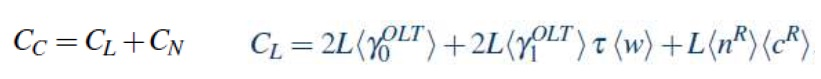
\includegraphics[width=\textwidth]{CAPEX}
  \caption{First function is CAPEX cost, second is cost of the links}
\end{figure}

\begin{figure}[h!]
  \centering
  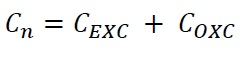
\includegraphics[scale=1]{CAPEX2}
  \caption{This function represent the cost of the nodes}
\end{figure}

We will also need a price list that we can see below.

\begin{figure}[h!]
  \centering
  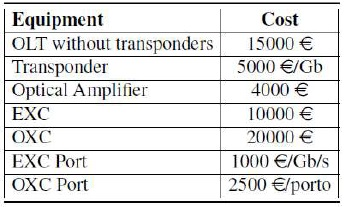
\includegraphics[scale=1]{TabValor}
  \caption{Table with costs}
\end{figure}

Finally we will calculate the CAPEX values for the various situations mentioned.

\subsection{Opaque with 1+1 Protection}
First we will present the scenario of little traffic and then in the case of a lot of traffic.
To know the value of CAPEX we will have to first calculate the value of the cost of the links and then the cost of the nodes.

\textbf{First scenario:}

Through the table, of auxiliary calculations and MatLab the value of the cost of the links is:

Cost link = 24 336 000 euros

Again, through the table, of auxiliary calculations and MatLab the value of the cost of the nodes is:

Cost node = 5 860 000 euros

Finally, for this scenario the cost of CAPEX is:

CAPEX = 30 196 000 euros

\textbf{Second scenario:}

Cost link = 191 336 000 euros

Cost node = 48 260 000 euros

CAPEX = 239 596 000 euros

\subsection{Transparent with 1+1 Protection}
Again, the first we will present the little traffic and then the lot of traffic.
To know the value of CAPEX we will have to first calculate the value of the cost of the links and then the cost of the nodes.

\textbf{First scenario:}

Through the table, of auxiliary calculations and MatLab the value of the cost of the links is:

Cost link = 44 336 000 euros

Again, through the table, of auxiliary calculations and MatLab the value of the cost of the nodes is:

Cost node = 2 515 000 euros

Finally, for this scenario the cost of CAPEX is:

CAPEX = 46 851 000 euros

\textbf{Second scenario:}

Cost link = 391 336 000 euros

Cost node = 21 445 000 euros

CAPEX = 412 781 000 euros

\subsection{Translucent with 1+1 Protection}

\section{Heuristics}

